% This is LLNCS.DOC the documentation file of
% the LaTeX2e class from Springer-Verlag
% for Lecture Notes in Computer Science, version 2.4
\documentclass{llncs}
\usepackage{llncsdoc}
\usepackage{amsmath}

\usepackage{graphicx}
\graphicspath{ {images/} }

% pour les accents utilisés en français 
\usepackage[utf8]{inputenc}
\usepackage[T1]{fontenc}
\usepackage[french]{babel}
\usepackage[hiperref]{}

%
\begin{document}
\markboth{\LaTeXe{} Class for Lecture Notes in Computer
Science}{\LaTeXe{} Class for Lecture Notes in Computer Science}
\thispagestyle{empty}
\begin{flushleft}
\LARGE\bfseries Rapport de stage\\[2cm]
\end{flushleft}
\rule{\textwidth}{1pt}
\vspace{2pt}
\begin{flushright}
\Huge
\begin{tabular}{@{}l}
Contrôle du mouvement\\
sur support mou\\
ou liquide\\[6pt]
{\Large Carensac Samuel}
\end{tabular}
\end{flushright}
\rule{\textwidth}{1pt}
\vfill
%\begin{flushleft}
%\large\itshape
%\begin{tabular}{@{}l}
%{\Large\upshape\bfseries Springer}\\[8pt]
%Berlin\enspace Heidelberg\enspace New\kern0.1em York\\[5pt]
%Barcelona\enspace Budapest\enspace Hong\kern0.2em Kong\\[5pt]
%London\enspace Milan\enspace Paris\enspace\\[5pt]
%Santa\kern0.2em Clara\enspace Singapore\enspace Tokyo
%\end{tabular}
%\end{flushleft}
%
\newpage
\tableofcontents
\newpage
%
\section{Résumé}
%
A rédiger en dernier
contexte 1 phrase
présenter le vérou 1 phrase
et comment il a été résolu 1/2 phrase
résultat 1 phrase
%
\section{Introduction}
%
1/ 1.5 page (à faire à la fin) abstract en écrivant +, sans les résultats et sans présenter précisément la méthode
Contexte
Problématique
Finir par le plan du document

%%%%%%%%%%%%%%%%%%%%%%%%%%%%%%%%%%%%%%%%%%%%%%%%
%%%%%%%%%%%%%%%%%%%%%%%%%%%%%%%%%%%%%%%%%%%%%%%% 

%
\section{Etat de l'art}
%
\subsubsection{Animation de personnages humains} 
Dans le cadre de l'animation de personnages on dispose d'un squelette composé de corps solides relié par des jointures permettant un certain nombre de degrés de libertés entre ces derniers. Il existe deux catégories de méthodes d'animation. La première, l'animation cinématique, décrit simplement les trajectoires des articulations au cours du temps. Bien que facile à réaliser cette méthode possède le défaut de rendre les interactions avec un environnement dynamique très compliquées. La seconde catégorie, l'animation basée physique, aborde le problème sous un tout autre angle. Cette fois –ci on ne déplacera pas directement les éléments du squelette mais on utilisera des interactions physiques pour les manipuler. On peut classer les interactions avec le squelette dans quatre catégories \cite{geijtenbeek2012interactive}: \newline
\begin{itemize}
\item{L'application de moments au niveau des jointures. Le principe est d'appliquer des moments au niveau des jointures pour faire se déplacer les éléments relativement entre eux suivant les degrés de liberté.}
\item{La seconde consiste à appliquer des forces directement sur les différents corps solide pour les animer. Cependant, un personnage réel no possédant pas la possibilité d'effectuer ce genre d'action, les résultats obtenus peuvent sembler surnaturels. Cette technique a d'ailleurs été surnommé "hand-of-god" \cite{van1995guided}. }
\item{La dernière méthode consiste à considérer des force comme la seconde méthode à la différence que celle-ci seront simulée à l'aide de moments sur les différentes articulations concernées. Cette méthode permet donc de simuler une force tout en gardant un résultat réaliste. On la retrouve notamment dans le cadre de contrôle de vitesse et d'équilibre \cite{coros2010generalized}.}
\end{itemize}

Pour permettre l'animation du squelette de manière à obtenir les déplacements désirés, des systèmes hauts niveau sont créés \cite{geijtenbeek2012interactive}. Ces système prendront en compte des paramètres de haut niveau tel que la vitesse et la posture et les convertiront en interactions avec le squelette définies ci-dessus. 

\subsubsection{Contrôle dans l'espace des joints} 
Ce type de méthode se base sur un système similaire à l'animation cinématique. L'utilisateur spécifie une série de positions désirées représentant le mouvement et le système tentera de suivre ces positions dans la limite du possible. A ceci s'ajoute des contrôleurs de feedback qui affecteront des moments supplémentaires suivant des règles intégrées au modèle.
\begin{figure}[h]
\centering
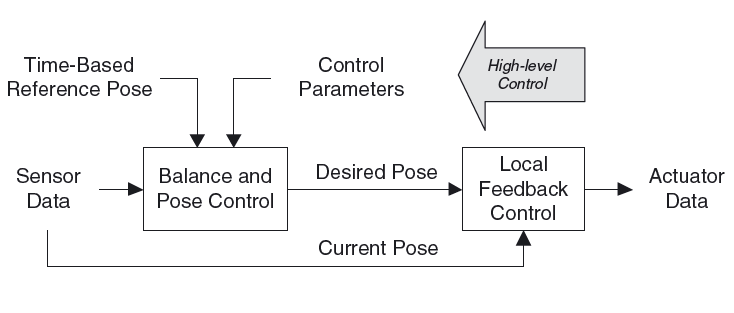
\includegraphics[scale=0.5]{joint_space_motion_control.png}
\caption{exemple de contrôleur dans l'espace des joints \cite{geijtenbeek2012interactive}}
\label{fig:joint_space_motion_control}
\end{figure}



Bien qu'il existe plusieurs méthodes permettant de suivre les positions spécifiées (antagonist feedback \cite{neff2002modeling}, non-linear force field \cite{mussa1997nonlinear}), la méthode la plus commune est le "proportionnal-derivative control" (PD-control). Un PD-contrôleur calcule un torque pour chaque articulation linéairement proportionnel à la différence entre l'état actuel et l'état désiré. Il prend en compte la différence entre les angles mais aussi la différence entre les vitesses angulaires 
\[
\tau=k_p(\theta_d - \theta) + k_v(\dot{\theta_d} - \dot{\theta})
\]

Parmi les systèmes basés sur un PD-contrôleur on trouve notamment le SIMBICON \cite{yin2007simbicon}. Le modèle est basé sur une machine à état finit. Chaque état est définit par une série de poses qui définiront les poses désirées au cours du mouvement. La transition d'un état à un autre peut s'effectuer après un certain temps ou bien lors d'un nouveau contact entre un pied et le sol. La spécification des poses clef possèdent quelques spécificités propres au SIMBICON. Les angles des articulations sont exprimé dans une repère local à l'exception de l'articulation entre le basin et le dos et de celle de la hanche de balance sont exprimées dans le repère du monde. Enfin la hanche d'appuis ne possède pas de positions cibles. Les moments à appliquer sur celle-ci sont déterminés de manière à obtenir le moment désiré sur le pelvis sans avoir recours à des forces extérieures.
\begin{figure}[h]
\centering
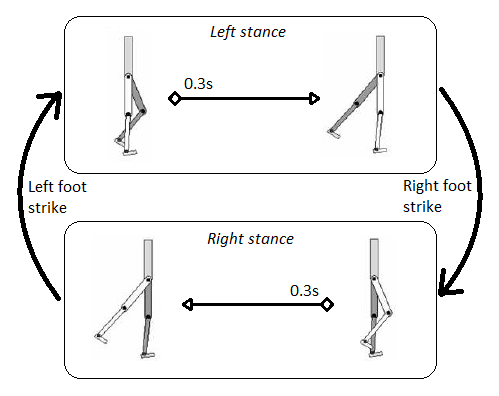
\includegraphics[scale=0.5]{state_machine.png}
\caption{exemple de machine à état pour la marche \cite{yin2007simbicon}}
\label{fig:state_machine}
\end{figure}


Le défaut du PD-contrôleur est qu'il est nécessaire de connaitre les bonnes valeurs pour les gains si l'on veut obtenir un résultat correct. Des gains trop faibles ne permettrait pas de suivre le mouvement définit. Des gains trop forts provoqueraient un mouvement saccadé et des possibles oscillations autour de la position désirée. On peut déterminer les bons paramètres par une série d'essais successifs mais cela ne permettrait pas d'obtenir un système robuste à des variations de géométrie dans le squelette. Pour pallier à ce problème le SIMBICON utilise un système de feedforward \cite{yin2007simbicon} sur les moments des articulations permettant ainsi d'obtenir une partie des moments nécessaire sans avoir à utiliser des gains élevés. Il existe d'autres méthodes permettant de calculer automatiquement une partie des moments. On trouve notamment un système de compensation de gravité \cite{coros2010generalized}. Ce système calcule des forces virtuelles compensant la gravité sur chaque partie du squelette.


\subsubsection{Maîtrise de l'équilibre au cours de la marche}
Définit tel quel le système ne permettrait pas de supporter des interactions avec l'environnement qui résulteraient en un déséquilibre. Pour pallier à ce problème le SIMBICON ajoute un système de balance feedback sur la hanche de balance et le pied d'appuis. Le principe est de modifier les angles cibles en fonction de la vitesse du centre des masses et de la distance entre celui-ci et le pied d'appuis. 
\[
\theta_d=\theta_d0 + c_d*d + c_v*v 
\]

Ce système permet d'obtenir un placement du pied intelligent qui maintient le personnage dans un équilibre stable. Parmi les autres systèmes de placement intelligent du pied on trouve l'utilisation d'un modèle du pendule inversé (IPM) \cite{kajita20013d,coros2010generalized}. En plus de permettre l'équilibre l'IPM possède l'avantage de pouvoir complètement définir le mouvement de la marche humaine utilisant des paramètres plus haut niveau tel que la hauteur des pas. Un avantage majeur d'un tel système est que l'on obtient une définition indépendante des caractéristiques physique du squelette offrant ainsi une grande flexibilité. Bien que très performant l'utilisation d'un IPM limite le déplacement à de la marche. De plus l'utilisation d'un IPM pour générer le mouvement complet de la jambe de balance limite grandement les styles de déplacement possibles.

\subsubsection{Contrôle de la vitesse}
Parmi les paramètres de haut niveau disponible à l'utilisateur on trouve le contrôle de la vitesse. Dans la version originale du SIMBICON la vitesse désirée est obtenue à l'aide d'une stratégie d'évolution. Le principe est de faire varier les positions cibles jusqu'à ce que l'on obtienne la vitesse voulue. Une amélioration du système \cite{coros2009robust} apporte la possibilité d'avoir plusieurs sets d'état. Le principe est d'avoir des sets généraux (i.e. marche avant, marche arrière, …) et de faire des combinaisons de ces états pour obtenir des états intermédiaires. Cela permet non seulement d'avoir une vitesse variable mais aussi de pouvoir changer de vitesse sans avoir à redémarrer le contrôleur. Plus récemment, un système un système appliquant une force virtuelle pour accélérer ou ralentir le personnage a été présentée \cite{coros2010generalized}. La force à appliquer est calculée à l'aide d'un PD-contrôleur se basant sur la vitesse du personnage. Ce système permet d'avoir un contrôle fin de la vitesse. Cette méthode de contrôle a été utilisée de manière intensive dans le but de conserver l'équilibre dans le cadre de déplacement dans une position statique \cite{geijtenbeek2012simple}. Cependant ce système ne permet pas de suivre correctement les vitesses si les poids du contrôler sont incorrect. Particulièrement si l'on place le personnage dans un milieu entravant son déplacement il serait nécessaire de retrouver les gains adaptés, si donné que ces gains existent. De plus l'application d'une force virtuelle reste limitée par les valeurs maximales des moments aux articulations. Ce qui veux dire que si le milieu gène beaucoup le mouvement, cette stratégie de contrôle devient invalide.

\subsubsection{Contrôle du mouvement en milieu aquatique}
La simulation d'interactions entre un personnage et un milieu liquide a déjà été effectuée. La plupart des travaux placent le personnage en milieu aqueux \cite{yang2004layered,kwatra2010fluid,tan2011articulated,si2014realistic}. On trouve également des articles utilisant un fluide pour simuler l'effet du vent sur le personnage \cite{lentine2011creature}. Cependant ces contrôleurs sont utilisés pour simuler de la nage et non de la marche. Dans les articles discutant des simulations de vent le personnage est entièrement immergé dans le fluide \cite{lentine2011creature}. De plus dans ce genre de situation l'effet de la poussée d'Archimède est ignoré. Dans le cadre de la simulation de l'eau de nombreux articles se servent d'un modèle basé sur les équations de Navier Stockes \cite{stam1999stable} avec une représentation eulérienne \cite{si2014realistic}. Le défaut est que ces systèmes ne permettent pas une simulation en temps réel. D'autres approches se contentent de modéliser l'eau à travers des forces extérieures calculées à l'aide d'équation simples \cite{yang2004layered}.

\subsubsection{Biomécanique de la marche en milieu aquatique}
La marche en milieu aquatique a été le sujet de plusieurs études dans le milieu de la biomécanique \cite{barela2006biomechanical,chevutschi2009comparison,orselli2011joint,miyoshi2005functional}. Certains de ces travaux travaillent sur les différences provoquées par la présence de l'eau \cite{barela2006biomechanical}. Cependant ces travaux utilisent des niveaux d'eau se situant au-dessus du niveau du processus xiphoïde. C’est-à-dire que l'impact de l'eau sur le torse et toujours présent ce qui modifie fortement les résultats par rapport à notre situation.

%%%%%%%%%%%%%%%%%%%%%%%%%%%%%%%%%%%%%%%%%%%%%%%%
%%%%%%%%%%%%%%%%%%%%%%%%%%%%%%%%%%%%%%%%%%%%%%%% 

\begin{figure}[h]
\centering
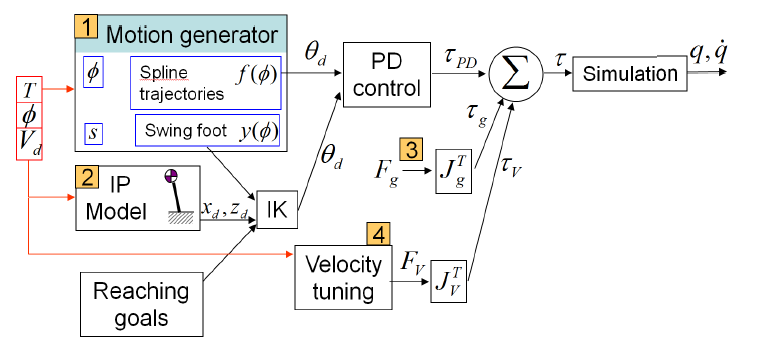
\includegraphics[scale=0.5]{system_overview.png}
\caption{schéma récapitulatif du contrôleur //celui-ci est pris de coros 2010, je n'ai pas encore fait le mien}
\label{fig:shema_controler}
\end{figure}

%
\section{Modélisation des fluides}
%
De manière à conserver une exécution en temps réel, le modèle utilisé se base sur les formules de base de dynamique des fluides. La poussée d'Archimède est calculée à partir du volume immergé de la représentation physique du squelette. L'influence du déplacement du personnage à l'intérieur de fluide n'a pas été considérée.
%
\subsection{Forces hydrodynamiques}
%
La résistance du fluide est calculée à partir de la formule suivante:
\[
F_D=\frac{1}{2} \rho v^3 A_n C_d
\]


Avec \(C_d\) le coefficient de résistance, \(\rho\) la densité du fluide, \(A_n\) la surface en vue du polygone et \(v\) la vitesse du polygone. La vitesse n'étant pas constante en tout point d'un polygone nous utilisons un découpage en éléments finis de la surface des polygones pour effectuer nos calculs.

La viscosité du fluide est implémentée à travers un coefficient 
\[
F=F_D*\mu
\]
Avec \(\mu\) la viscosité du fluide.
%
\subsection{Poussée d'Archimède}
%
La poussée d'Archimède est calculée à l'aide de la formule du même nom:
\[
P_A=-V_i \rho g
\]
Le volume immergé \(V_i\) étant déterminé soit par l'utilisation des formules existantes (sphères, cylindres) soit par une représentation du polygone en voxels (prismes)
%
\section{Contrôle du mouvement}
%
Comme présenté par la figure \ref{fig:shema_controler}, le système de contrôle du mouvement est composé de 3 blocs principaux: suivit des poses clef, conservation de l'équilibre et suivit de la vitesse. Voici une vision globale du fonctionnement du système.

Chaque joint possède une trajectoire à suivre pour chaque degré de liberté. Ces trajectoires sont déterminées à partir d'un certain nombre de points clef et les valeurs intermédiaires sont déterminées à l'aide de splines Catmull-Rom. Les joints ayant une influence sur la vitesse possèdent un set de trajectoires chacune correspondant à une vitesse. Suivant la vitesse le système calcule une combinaison des deux trajectoires des deux vitesses les plus proches. Les trajectoires de la jambe de balance sont déterminées dynamiquement à partie de la trajectoire désirée pour le pied de balance.
Pour permettre l'utilisation de gains faibles dans le PD-contrôleur nous utilisons le système de compensation de gravité présenté par \cite{coros2010generalized}. Ce système permet de calculer indépendamment une partie des moments nécessaire au mouvement d'alléger la charge du PD-contrôler.

La conservation de l'équilibre est réalisée par un placement du pied intelligent déterminé par un modèle de pendule inversé (IPM). Pour aider ce système les articulations de la hanche et du pied d'appuis possèdent des modèles de feedback corrigeant la position du personnage.

Le contrôle de la vitesse est obtenu à l'aide d'une force virtuelle similaire à celle utilisée par \cite{coros2010generalized}. Ce système a été amélioré pour prendre en compte les variations de vitesse interne à un pas. Ce système est aidé par une altération des résultats de l'IPM permettant d'accélérer ou de ralentir le personnage. Ces deux système sont contrôlés par du feedback et ne nécessitent aucun paramétrage.
%
\subsection{Modélisation du personnage}
%
\begin{figure}[h]
\centering
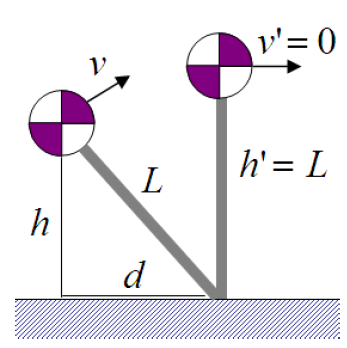
\includegraphics[scale=0.5]{IPM.png}
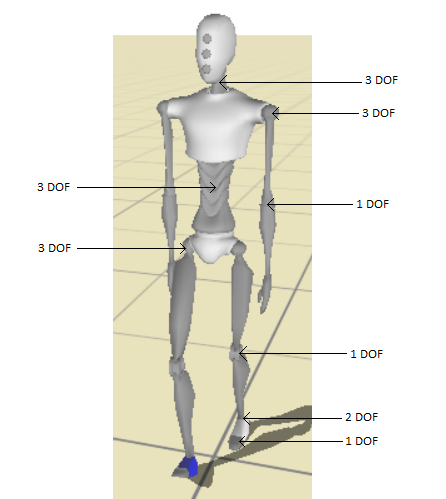
\includegraphics[scale=0.5]{img_dof.png}
\caption{A gauche, modèle du pendule inversé \cite{coros2010generalized}. A droite, degrés de liberté internes}
\label{fig:dof}
\end{figure}

Le personnage utilisé est composé de corps solides simples (sphères, cylindres et prismes). Celui-ci est composé des 28 degrés de liberté interne présentés dans la figure \ref{fig:dof} plus 6 degrés de liberté externe (position et orientation).

%
\subsection{Générateur de mouvement}
\begin{figure}[h]
\centering
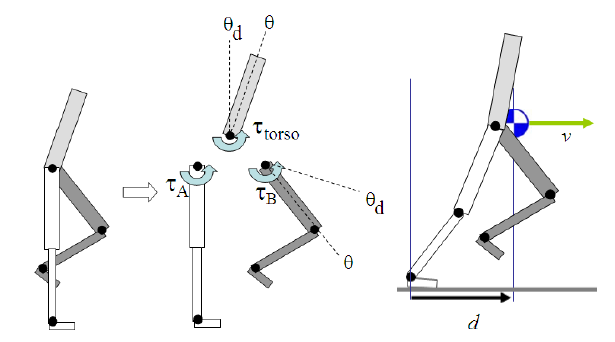
\includegraphics[scale=0.5]{stance_torque_and_v_and_d.png}
\caption{A gauche, calcul des moments sur le pelvis \cite{yin2007simbicon}. A droite, représentation des variables \(d\) et \(v\) \cite{yin2007simbicon}.}
\label{fig:torques_pelvis}
\label{fig:d_and_v}
\end{figure}
Le générateur de mouvement prend comme entrée les trajectoires définies par l'utilisateur pour chaque degré de liberté à l'exception de la jambe de balance et de la hanche d'appuis. Ces trajectoires indiquent les angles désirés à un instant donné du mouvement. Les angles sont définis comme les angles relatif entre le polygone parent et le polygone enfant de chaque articulation à l'exception des angles du pelvis et des hanches. Les angles du pelvis et de la hanche de balance sont définis dans le repère du personnage. Ce repère est similaire au repère du monde à l'exception d'une rotation sur l'axe y (axe vertical) permettant de garder l'axe z dans la direction que face le personnage. Cette rotation est définie par une variable de "heading" qui est utilisée pour contrôler la direction de marche du personnage. Les trajectoires sont des courbes de la phase \(\phi \) d'un pas (\(\phi \in [0,1] \)). L'alternation gauche droite des pas est gérée en utilisant le symétrique des trajectoires. Les courbes sont définies par un nombre arbitraire de points clefs choisis par l'utilisateur et les valeurs pour les positions intermédiaires sont déterminées à l'aide de splines Catmull-Rom.
Le générateur de mouvement convertit ces angles désirés en moments aux articulations en utilisant un PD-contrôleur:
\[
\tau=k_p(\theta_d - \theta) + k_v(\dot{\theta_d} - \dot{\theta})
\]
Il est commun de voir que la position atteinte par le système soit très différente de la position demandée, particulièrement avec la présente d'un milieu aquatique. 

Le générateur de mouvement est composé d'une machine à états similaire à celle utilisée par \cite{yin2007simbicon}. Le système change d'un état au suivant à chaque fois que le pied de balance touche le sol. L'utilisateur définit une durée de temps \(T \) pour chaque pas. La phase \(\phi \) à un instant \(t \) après le changement d'état est déterminée par \(\phi=\frac{t}{T}\) .

Les trajectoires désirées pour les éléments composant la jambe de balance sont déterminées dynamiquement par l'utilisation d'un IPM (section \ref{sec:IPM}) et une définition de la trajectoire du pied de balance. Le système détermine la position du pied en choisissant soit la position définit par l'utilisateur soit celle indiquée par l'IPM. Le choix est effectué suivant des règles définies dans la section présentant l'IPM.

Le moment \(\tau_b \) à appliquer à la hanche d'appui est calculé de manière à ce que le moment total sur le pelvis corresponde au moment permettant d'obtenir l'orientation définie par l'utilisateur. Ce moment \(\tau \) désiré est déterminé par le PD-contrôleur en prenant pour angle cible la somme de l'angle définit dans la trajectoire du pelvis plus l'angle de heading (figure \ref{fig:torques_pelvis}).
\[
\tau_b=\tau - \tau_a - \tau_{torso}
\]
Avec \(\tau_a \) le moment appliqué sur la hanche de balance et \(\tau_{torso} \) le moment appliqué à l'articulation entre le pelvis et le torse.

Le générateur de mouvement possède également la capacité d'adapter les trajectoires des articulations en utilisant la combinaison de plusieurs trajectoires définies par l'utilisateur. Le principe est de faire la combinaison des états optimaux pour des environnements différents (vitesse différente, présence d'un liquide). Ce système est présenté dans la section \ref{sec:multi_state}

\subsubsection{Compensateur de gravité}
\label{sec:jacob}
\begin{figure}[h]
\centering
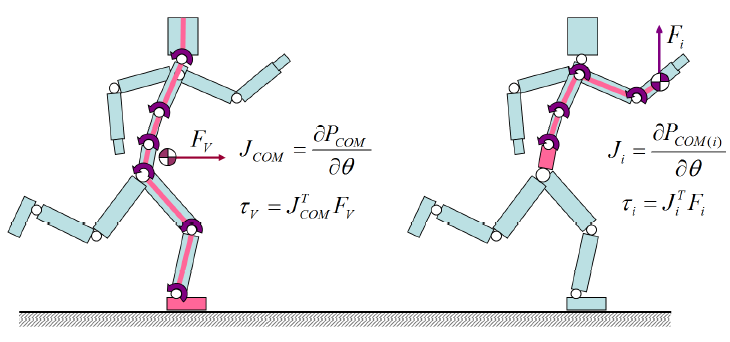
\includegraphics[scale=0.5]{shema_jacobians.png}
\caption{A gauche, jacobienne utilisée pour le contrôle de vitesse. A droite, jacobienne utilisée pour la compensation de gravité. \cite{coros2010generalized} }
\label{fig:jacob}
\end{figure}

Le compensateur de gravité permet l'utilisation de gains faibles dans le PD-contrôleur et ainsi éviter la création de mouvements robotiques. Notre système est très similaire à celui présenté par \cite{coros2010generalized}. Le principe est de calculer pour chaque partie du personnage une force virtuelle compensant la gravité. Donc pour chaque polygone nous appliquons une force \(F_{GC}=-mg\) au centre des masses, le signe négatif indiquant une force vers le haut. Cette force est ensuite convertie en moment pour chaque articulation se trouvant dans la chaine reliant le point d'application de la force et le pelvis \(\tau=J_i^T F\). \(J_i\) est la transposée de la jacobienne de la chaine reliant le pelvis et le point d'application de la force.
La jacobienne d'une chaine de \(k\) articulation contient les informations indiquant l'impact d'une rotation de chaque degré de liberté de la chaine sur le point final de la chaine
\[
J(p)^T =\begin{bmatrix}
\frac{\partial p_x}{\partial \alpha_1} & \frac{\partial p_y}{\partial \alpha_1} & \frac{\partial p_z}{\partial \alpha_1} \\
\vdots & \vdots & \vdots \\
\frac{\partial p_x}{\partial \alpha_n} & \frac{\partial p_y}{\partial \alpha_n} & \frac{\partial p_z}{\partial \alpha_n} \\
\end{bmatrix}
\]
Chaque \(\frac{\partial p_x}{\partial \alpha_i}\) peut être calculé par le produit vectoriel entre l'axe de la rotation et le vecteur allant de l'articulation \(i\) et le point d'application
\[
J(p)_i ^T =\begin{bmatrix}
\frac{\partial p_x}{\partial \alpha_i} & \frac{\partial p_y}{\partial \alpha_i} & \frac{\partial p_z}{\partial \alpha_i} \\
\end{bmatrix}
= (\alpha_i \times (p-p_i))^T
\]
Donc la force à appliquer à chaque articulation i correspond à:
\[
\tau = (\alpha_i \times (p-p_i))^T F
\]
Cette méthode de compensation de gravité est appliquée à tous les solides du squelette excepté ceux composant la jambe d'appuis.

Nous avons modifié légèrement ce système pour permettre la prise en compte d'un milieu liquide. Cette modification consiste à calculer les valeurs de la poussée d'Archimède sur chaque membre du personnage et de soustraire celle-ci à la force virtuelle à appliquer. Il parait intéressant de noter qu'il ne suffit pas simplement de diminuer l'intensité de la force à appliquer. En effet suivant la modélisation des membres du personnage, il est possible, et même fortement probable, que la densité soit variable à l'intérieur de ceux-ci. De ce fait le point d'application de la force compensant la gravité et celui de la poussée d'Archimède seront différent, ce qui nous oblique à déterminer le point d'application de la force finale \(F=F_{GC}- P_A\).

\subsection{Conservation de l'équilibre}
%
L'équilibre du personnage est obtenu par le placement intelligent du pied à l'aide d'un modèle de pendule inversé (IPM) et de fonctions de feedback sur certaines articulations (balance feedback). Les systèmes de contrôle de vitesse (section\ref{sec:speed_control}) permettent également un maintien de l'équilibre du fait qu'ils maintiennent le système autour d'une vitesse stable. 
%
\subsubsection{Modèle du pendule inversé}
%
\label{sec:IPM}

\begin{figure}[h]
\centering
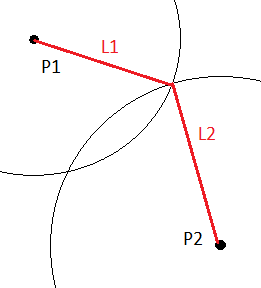
\includegraphics[scale=0.5]{inv_kin_basic.png}
\caption{schéma présentant comment trouver l'articulation séparant deux membres à partir des positions des extrémités *légende à revoir, schéma à refaire*}
\label{fig:inv_kin}
\end{figure}

Pouvoir déterminer dynamiquement la position optimale pour conserver l'équilibre est un très grand avantage pour obtenir un contrôleur robuste aux interactions avec l'environnement. Pour déterminer la position p(x,y) du prochain pas, nous utilisons un modèle de pendule inversé. Nous utilisons le même modèle que \cite{coros2010generalized} et considérons une longueur de jambe constante.
Le principe de l'IPM est de partir du constat que la somme de l'énergie potentielle de pesanteur et de l'énergie cinétique reste constante peu importe la position du pendule (figure \ref{fig:inv_kin}). 
\[
\frac{1}{2}mv^2+mgh=\frac{1}{2}mv'^2+mgh'
\]
Si l'on considère que lors de la position d'équilibre (position verticale) nous désirons une vitesse nulle nous pouvons simplifier l'équation avec les variables suivantes \(v'=0\) et \(h'=L=\sqrt{h^2+d^2}\). On peut ainsi déterminer la valeur de \(d\).
\[
d=v\sqrt{\frac{h}{g}+\frac{v^2}{4g^2}}
\]
Pour permettre d'avoir un résultat conservant une vitesse proche de la vitesse désirée \(V_d\) une altération des résultats de l'IPM est réalisé \(\Delta=\alpha V_d\). Ainsi une vitesse positive apporte une diminution de la longueur des pas provoquant une accélération et inversement une vitesse négative ralentit le personnage. Ce système est étendu à un système de feedback pour le contrôle précis de la vitesse (voir section \ref{sec:ipm_alt}).
Selon la vitesse de personnage il est possible que l'IPM nous donne des résultats impossible à atteindre c'est pourquoi la longueur des pas est limitée à \(d=0.6L\) avec \(L\) la longueur de la jambe.
La position effective du pied est calculée à l'aide d'une interpolation entre la position de départ du pied et la valeur retournée par l'IPM. La loi d'interpolation utilisée est une loi d'ordre 2:
\[
P_f=(1-\phi^2)*pos_{init}+\phi^2*p(x,y)
\]
La hauteur du pied au cours du pas est définie par l'utilisateur à l'aide d'une trajectoire.
Les angles désirés pour la hanche et le genou sont ensuite déterminés à l'aide de la cinématique inversé (voir figure \ref{fig:inv_kin}. Il reste un degré de liberté qui est fixé pour que la position du genou se trouve dans le plan de rotation de la hanche.

Bien que l'IPM soit intéressant il limite les possibilités de mouvement. Par exemple il rend impossible un mouvement définissant une trajectoire rectangulaire pour le pied comme l'on voit sur la figure *mettre nbr figure de la strip avec une marche carrée*. Ce genre de déplacement est important dans le cadre de notre étude car elles sont typiques de lieu ou la progression est beaucoup entravée (par exemple de la neige). Pour permettre l'observation de tels déplacements nous avons rajouté la possibilité de manuellement définir la position du pied au cours du pas. Cette définition manuelle est considérée temps que le personnage est dans la phase ascendante du pas \(V_{COM}(y)>0\) et qu'il n'est pas dans un état instable. Nous déterminons une instabilité du personnage si nous détectons une variation irrégulière du pattern de vitesse observé au cours d'un pas (voir la section \ref{sec:speed_virt_force}). Si un état instable est détecte nous utilisons le résultat de l'IPM pour la totalité du pas jusqu'à ce que nous retournions dans un état stable.

%
\subsubsection{Balance feedback}
%
Dans le cadre de ce feedback nous utilisons une loi linéaire fonction de \(d\) et de \(v\) pour altérer les angles désirés:
\[
\theta_d=\theta_d0 + c_d*d + c_v*v 
\]

Avec \(\theta_d\) l'angle qui sera utilisé par le PD-contrôleur, \(\theta_{d0}\) l'angle spécifié par les trajectoires, \(d\) la distance entre le centre des masses et le pied d'appuis et \(v\) (voir figure \ref{fig:d_and_v}) la vitesse de centre des masses.
Les gains \(c_d\) et \(c_v\) sont déterminés pendant la phase d'optimisation hors-ligne. 

Ce système est appliqué sur la cheville d'appuis. Il est utilisé pour obtenir une partie du moment nécessaire à appliquer ce qui permet de conserver des gains faibles. Il est important de signaler que ce n'est qu'une stratégie d'équilibre secondaire car la nécessité d'avoir des gains optimaux la rend très peu flexible. 
%
\subsection{Contrôle de vitesse}
%
\label{sec:speed_control}
Dans le cadre de ce projet, la capacité à marcher à une vitesse donnée est un critère primordial. De plus nous souhaitons obtenir un système qui sera robuste à la variation du milieu (présence ou non de liquide). Pour obtenir un tel résultat, nous utilisons une force virtuelle ainsi qu'un système d'altération des résultats de l'IPM.
%
\subsubsection{Contrôle de vitesse par force virtuelle}
%
\label{sec:speed_virt_force}
*mettre une img pr illustrer l'adaptation de la courbe et la détection des irrégularités*
Pour obtenir une vitesse désirée nous allons appliquer une force virtuelle horizontale qui accélèrera ou ralentira le personnage en déplaçant le centre des masses. Ce système est basé sur le système utilisé par \cite{coros2010generalized}.
Le principe est d'utiliser une PD-contrôler se basant sur la différence entre la vitesse actuelle du personnage et la vitesse désirée pour déterminer l'intensité de la force à appliquer. La force sera ensuite appliquée au centre des masses du personnage en calculant les torques nécessaires à l'aide de la méthode de la transposée jacobienne (voir section \ref{sec:jacob} ). La chaine de polygone considérés pour l'application de la force est la chaine reliant le torse au pied d'appuis (voir figure \ref{fig:jacob}). Les valeurs utilisées pour la jacobienne sont légèrement différentes de celles-ci utilisées précédemment. Cette fois nous utilisons la somme des vecteurs séparant les articulations pondérés par le poids du membre présent entre ces deux articulations.
\[
J(p) _n ^T =\frac{ \sum_{\substack{0<i\leq n}} ((P_i(x,y,z)-P_{i-1}(x,y,z))*M_i)}{M} 
\]
Avec \(M\) la somme des poids pour de tous les membres considérés par le système et \(P_i(x,y,z)\) la position de l'articulation \(i\) de la chaine, \(P_0(x,y,z)\) étant le point d'application de la force. Ceci nous permet d'accorder une importance plus grande aux articulations provoquant de grands changements dans la position de centre des masses. 

Il est facile d'observer que la vitesse de déplacement du centre des masses n'est pas constante au cours d'un pas. Cependant lorsque nous somme dans le cas d'un déplacement stable, ces variations de vitesse sont constantes à chaque pas. C'est pourquoi nous avons construit un système permettant d'apprendre cette courbe de variation de vitesse de manière à appliquer une force virtuelle plus adaptée. De manière similaire aux trajectoires des articulations cette courbe est définie comme une fonction de \(\phi\) et possède un nombre de point de référence arbitraire. Les valeurs entre les points de références sont également déterminées à l'aide de Catmull-Rom splines. Un nombre de 10 points de référence s'est montré être une valeur correcte.
Ce paragraphe explique de manière plus précise l'apprentissage de la courbe. Aux cours d'un pas nous relevons pour chaque point de référence la différence entre la valeur stockée dans la courbe et la valeur observée réellement. Si la variation moyenne observée est inférieur à une heuristique, nous adaptons les valeurs stockées pour les rapprocher des valeurs observées. Pour finir nous déterminons le ratio entre la vitesse moyenne demandée et la vitesse moyenne et nous modifions les points de la courbe de façon à ce que la nouvelle courbe définisse les valeurs à demander pour obtenir la vitesse voulue.

La présence de l'heuristique nous permet de détecter les variations irrégulières de la courbe de vitesse. Une fois la situation d'équilibre atteinte nous obtenons une courbe stable qui est caractéristique au déplacement constaté. Si l'on observe une variation de cette courbe cela veut dire qu'un élément est venu perturber le déplacement. Dans ce cas, nous déclarons au système que nous ne sommes plus dans un état stable ce qui adaptera la stratégie de déplacement jusqu'à ce que le mouvement redevienne stable. Une fois le mouvement redevenue stable nous recommençons à adapter la courbe de vitesses.
%
\subsubsection{Altération des résultats de l'IPM}
\label{sec:ipm_alt}
%
*présenter le sys d'apprentissage du delta et les limites que l'on met à ce système et pourquoi*
%

\subsubsection{Système de combinaison d'états}
\label{sec:multi_state}
%
*présenter le sys de combinaison des états et dire sur quelles trajectoires je le fait et pourquoi*
% 
\subsection{Off-line optimisation}
%
*faire une mini intro disant que on l'util pr trouver des style de marche suivant des critères d'évolutions voulues (ex min contact avec le liquide, minimiser l'effort fourni)*
%
\subsubsection{Fonction objectif}
%
*faire un descriptif de chaque blocs de la méthode d'évaluation et dire que l'on util une pondération*
%
\subsubsection{Méthode d'évolution des paramètres}
%
*faire mini état de l'art de cma et dire qu'on l'utilise*
%



%%%%%%%%%%%%%%%%%%%%%%%%%%%%%%%%%%%%%%%%%%%%%%%%
%%%%%%%%%%%%%%%%%%%%%%%%%%%%%%%%%%%%%%%%%%%%%%%% 

%
\section{Résultats}
%
*donner paramètres, méthodologies utilisée pr les expériences, capacités système*
*faire un comparatif visuel des mouvement obtenus suivant le niv d'eau pr les diff combinaisons d'évaluations*
*faire une comparaison en désactivant les systèmes créés*
*si il y en a présenter lestruc qui peuvent être utilisé en tant que feed back*
*faire une partie limitation*

\section{Conclusion}
%
*faire une conclusion qui contient la partie travaux futur*
%

\section{References}
%

%
\nocite{*}
\bibliographystyle{splncs03}
\bibliography{references}
%
\end{document}
